%set the master document for easy compilation
%!TEX root = ../D3_5_3.tex

\section{F2.1: Manage\_TrackSideInformation\_Integration}

\subsection{Component Requirements}

\todo[inline]{Clarify detail for documentation with the trackMessages concept}


\begin{longtable}{p{.25\textwidth}p{.7\textwidth}}
\toprule
Component name			& Manage\_TrackSideInformation\_Integration \\
\midrule
Link to SCADE model		& {\footnotesize \url{https://github.com/openETCS/modeling/blob/master/model/Scade/System/ObuFunctions/ManageLocationRelatedInformation/BaliseGroup/Manage_TrackSideInformation_Integration/Manage_TrackSideInformation_Integration.etp}} \\
\midrule
SCADE designer			& Bernd Hekele, DB Netz AG \\
\midrule
Description				& The block ``Manage\_TrackSideInformation\_Integration'' is responsible for receiving Eurobalise telegrams and Euroradio messages from the API and performs several consistency checks on the inputs.\newline

The block collects the telegrams of balises in order to build balise group messages. Euroradio messages are always delivered as a whole message. On each message, a consistency check is performed, before the data is validated according to the driving direction of the train. In general, messages not designated for the current driving direction of the train are not forwarded to the further processing. After applying consistency checks, the data direction is validated. \\
\midrule
Input documents			& See subcomponents.\\
\midrule
Safety integrity level	& 4 \\
\midrule
Time constraints		& The component has to be able to receive balise telegrams and radio messages according to the ETCS \cite{subset-41} performance requirements). In highspeed traffic, a group of 8 balises must be read in about 250 msec. In addition, 1 message per sec. on the radio interface is to be expected.\\
\midrule
API requirements 		& Interfaces to this unit are defined in the API sections [BTM], [EURORADIO], [ODO].In these sections, also a detailed definition of the concepts implemented on those interfaces is documented.  \\
\bottomrule
\end{longtable}


\subsection{Interface}

An overview of the interface of component Manage\_TrackSideInformation\_Integration is shown in Figure~\ref{f:receiveAndCheckConsistencyArch}. The inputs and outputs are described in detail in Section~\ref{s:Manage_Trackside_inputs} respectively \ref{s:Manage_Trackside_outputs}. Subcomponents are described in Section~\ref{s:receivetrackdata_subcomponents}.

\begin{figure}
\center
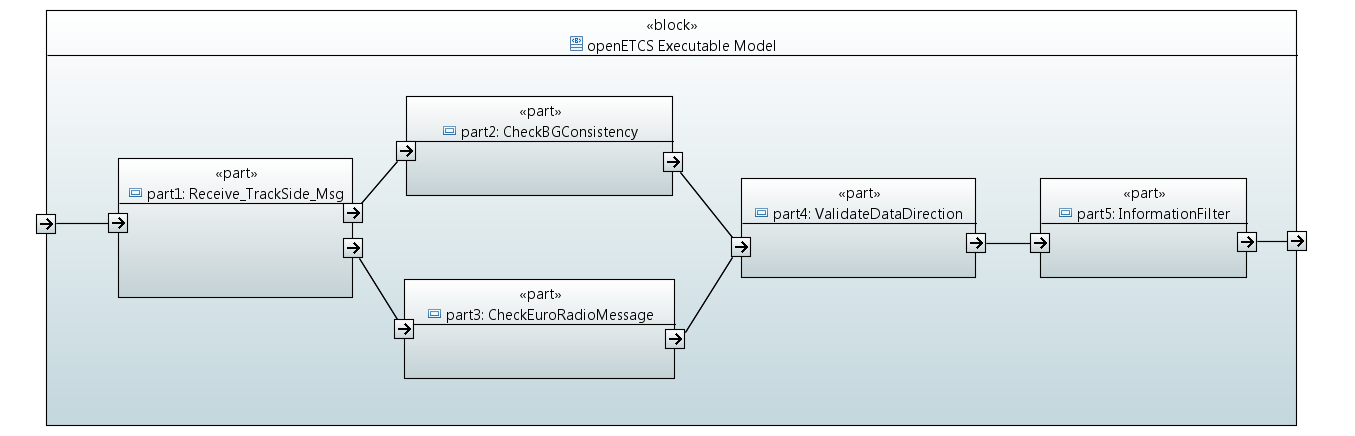
\includegraphics[width=\textwidth]{./images/Input-Messages4.PNG}
\caption{Manage\_TrackSideInformation\_Integration component SysML diagram.}\label{f:receiveAndCheckConsistencyArch}
\end{figure}


\subsubsection{Inputs}\label{s:Manage_Trackside_inputs}

\paragraph{fullChecks}

\begin{longtable}{p{.25\textwidth}p{.7\textwidth}}
\toprule
Input name				& fullChecks \\
\midrule
Description				& Indicates, if all checks on the message should be performed. \\
\midrule
Source					& This item is only relevant in verification phases. In a real system checks are always activated. \\ 
\midrule
Type					& bool \\
\midrule
Valid range of values	& 
\begin{description}
\item[true] All checks are performed.
\item[false] Component InformationFilter is deactivated.
\end{description} \\
\midrule
Behaviour when value is at boundary	& n/a \\
\midrule
Behaviour for values out of valid range	& n/a \\
\midrule
Behaviour when value is erroneous, absent or unwanted (i.e. spurious) & [Description of components behaviour when value is erroneous, absent or unwanted (i.e. spurious)] \\
\bottomrule
\end{longtable}


\paragraph{Receive\_trackSide\_Message}

\begin{longtable}{p{.25\textwidth}p{.7\textwidth}}
\toprule
Input name				& API\_trackSide\_Message \\
\midrule
Description				& Track side message received from the API. The API performs preprocessing of RTM and BTM messages and deliveres a maximum of a single message per cycle. The structure of this message is defined in the API [BTM] and [EURORADIO] sections.\\
\midrule
Source					& API \\ 
\midrule
Type					& API\_Msg\_Pkg::API\_TrackSideInput\_T \\
\midrule
Valid range of values	& [Complete list of valid values] \\
\midrule
Behaviour when value is at boundary	& [Description of components behaviour when input value is at boundary] \\
\midrule
Behaviour for values out of valid range	& [Description of components behaviour when input value is out of valid range] \\
\midrule
Behaviour when value is erroneous, absent or unwanted (i.e. spurious) & [Description of components behaviour when value is erroneous, absent or unwanted (i.e. spurious)] \\
\bottomrule
\end{longtable}


\paragraph{ActualOdometry}

\begin{longtable}{p{.25\textwidth}p{.7\textwidth}}
\toprule
Input name				& ActualOdometry \\
\midrule
Description				& Provided by the external odometry module of the train. It contains relative location information with inaccuracies. \\
\midrule
Source					& Odometer \\ 
\midrule
Type					& Obu\_BasicTypes\_Pkg::odometry\_T \\
\midrule
Valid range of values	& [Complete list of valid values] \\
\midrule
Behaviour when value is at boundary	& [Description of components behaviour when input value is at boundary] \\
\midrule
Behaviour for values out of valid range	& [Description of components behaviour when input value is out of valid range] \\
\midrule
Behaviour when value is erroneous, absent or unwanted (i.e. spurious) & [Description of components behaviour when value is erroneous, absent or unwanted (i.e. spurious)] \\
\bottomrule
\end{longtable}

\paragraph{reset}

\begin{longtable}{p{.25\textwidth}p{.7\textwidth}}
\toprule
Input name				& reset \\
\midrule
Description				& To delete all data stored in the module (e.g.~collected balise telegrams, which do not yet form a complete message), a reset input can be used. If the input is set to true, all data kept in the module is deleted and no input is accepted. \\
\midrule
Source					& Environment \\ 
\midrule
Type					& bool \\
\midrule
Valid range of values	& 
\begin{description}
\item[true] All data kept in the module is deleted and no input is accepted.
\item[false] No action. Data at input is accepted.
\end{description} \\
\midrule
Behaviour when value is at boundary	& [Description of components behaviour when input value is at boundary] \\
\midrule
Behaviour for values out of valid range	& [Description of components behaviour when input value is out of valid range] \\
\midrule
Behaviour when value is erroneous, absent or unwanted (i.e. spurious) & [Description of components behaviour when value is erroneous, absent or unwanted (i.e. spurious)] \\
\bottomrule
\end{longtable}

\paragraph{trainPosition}

\begin{longtable}{p{.25\textwidth}p{.7\textwidth}}
\toprule
Input name				& trainPosition \\
\midrule
Description				& Contains the current position of the train. \\
\midrule
Source					& CalculateTrainPosition \\ 
\midrule
Type					& TrainPosition\_Types\_Pck::trainPosition\_T \\
\midrule
Valid range of values	& \\
\midrule
Behaviour when value is at boundary	& [Description of components behaviour when input value is at boundary] \\
\midrule
Behaviour for values out of valid range	& [Description of components behaviour when input value is out of valid range] \\
\midrule
Behaviour when value is erroneous, absent or unwanted (i.e. spurious) & [Description of components behaviour when value is erroneous, absent or unwanted (i.e. spurious)] \\
\bottomrule
\end{longtable}

\paragraph{modeAndLevel}

\begin{longtable}{p{.25\textwidth}p{.7\textwidth}}
\toprule
Input name				& modeAndLevel \\
\midrule
Description				& Provides the current level and mode of the EVC. \\
\midrule
Source					& ModeAndLevel \\ 
\midrule
Type					& BG\_Types\_Pkg::ModeAndLevelStatus\_T \\
\midrule
Valid range of values	& [Complete list of valid values] \\
\midrule
Behaviour when value is at boundary	& [Description of components behaviour when input value is at boundary] \\
\midrule
Behaviour for values out of valid range	& [Description of components behaviour when input value is out of valid range] \\
\midrule
Behaviour when value is erroneous, absent or unwanted (i.e. spurious) & [Description of components behaviour when value is erroneous, absent or unwanted (i.e. spurious)] \\
\bottomrule
\end{longtable}


\paragraph{tNvContact}

\begin{longtable}{p{.25\textwidth}p{.7\textwidth}}
\toprule
Input name				& tNvContact \\
\midrule
Description				& For monitoring the safe radio connection, this national value is needed as an input. \\
\midrule
Source					& Database \\ 
\midrule
Type					& Obu\_BasicTypes\_Pkg::T\_internal\_Type \\
\midrule
Valid range of values	& [Complete list of valid values] \\
\midrule
Behaviour when value is at boundary	& [Description of components behaviour when input value is at boundary] \\
\midrule
Behaviour for values out of valid range	& [Description of components behaviour when input value is out of valid range] \\
\midrule
Behaviour when value is erroneous, absent or unwanted (i.e. spurious) & [Description of components behaviour when value is erroneous, absent or unwanted (i.e. spurious)] \\
\bottomrule
\end{longtable}


\paragraph{lastRelevantEventTimestamp}

\begin{longtable}{p{.25\textwidth}p{.7\textwidth}}
\toprule
Input name				& lastRelevantEventTimestamp \\
\midrule
Description				& For monitoring the safe radio connection, it is necessary that the time between two packets is less than the value of {T\_NVCONTACT}.\newline
In situations like level-changes or announced radio holes, not the timestamp of the last message is relevant for comparison, but the timestamp of the last relevant event. This can for example be the timestamp of the level change or the timestamp of the moment, when the train was passing the end of the radiohole.\newline
For performing this check, the timestamp of the last relevant event is provided to the model as an {T\_internal\_Type}-type. \\
\midrule
Source					& Database \\ 
\midrule
Type					& Obu\_BasicTypes\_Pkg::T\_internal\_Type \\
\midrule
Valid range of values	& [Complete list of valid values] \\
\midrule
Behaviour when value is at boundary	& [Description of components behaviour when input value is at boundary] \\
\midrule
Behaviour for values out of valid range	& [Description of components behaviour when input value is out of valid range] \\
\midrule
Behaviour when value is erroneous, absent or unwanted (i.e. spurious) & [Description of components behaviour when value is erroneous, absent or unwanted (i.e. spurious)] \\
\bottomrule
\end{longtable}


\paragraph{connectionStatus}

\begin{longtable}{p{.25\textwidth}p{.7\textwidth}}
\toprule
Input name				& connectionStatus \\
\midrule
Description				& Status information about the radio connection. The information is needed to perform the timing check, which depends on the connection state. \\
\midrule
Source					& ManageRadioCommunication \\ 
\midrule
Type					& Radio\_Types\_Pkg::sessionStatus\_Type \\
\midrule
Valid range of values	& 
\begin{description}
\item[DISCONNECTED] The OBU is currently not connected to a RBC.
\item[CONNECTING] The OBU is currently connecting to the RBC. Received messages belong to the process of establishing a connection.
\item[CONNECTION\_ESTABLISHED] The connection to the RBC is established.
\end{description} \\
\midrule
Behaviour when value is at boundary	& [Description of components behaviour when input value is at boundary] \\
\midrule
Behaviour for values out of valid range	& [Description of components behaviour when input value is out of valid range] \\
\midrule
Behaviour when value is erroneous, absent or unwanted (i.e. spurious) & [Description of components behaviour when value is erroneous, absent or unwanted (i.e. spurious)] \\
\bottomrule
\end{longtable}


\paragraph{inSupervisingRbcId}

\begin{longtable}{p{.25\textwidth}p{.7\textwidth}}
\toprule
Input name				& inSupervisingRbcId \\
\midrule
Description				& For the subcomponent InformationFilter, the information which radio messages are sent by the supervising RBC is needed. To recognize these messages, the identifier of the supervising RBC is needed. \\
\midrule
Source					& Database \\ 
\midrule
Type					& int \\
\midrule
Valid range of values	& [Complete list of valid values] \\
\midrule
Behaviour when value is at boundary	& [Description of components behaviour when input value is at boundary] \\
\midrule
Behaviour for values out of valid range	& [Description of components behaviour when input value is out of valid range] \\
\midrule
Behaviour when value is erroneous, absent or unwanted (i.e. spurious) & [Description of components behaviour when value is erroneous, absent or unwanted (i.e. spurious)] \\
\bottomrule
\end{longtable}


\paragraph{inAnnouncedBGs}

\begin{longtable}{p{.25\textwidth}p{.7\textwidth}}
\toprule
Input name				& inAnnouncedBGs \\
\midrule
Description				& Provides information about balise groups which will be passed by the train soon. This information is generated by Calculate Train Position based on the linking information received from trackside. \\
\midrule
Source					& CalculateTrainPosition \\ 
\midrule
Type					& TrainPosition\_Types\_Pck::positionedBGs\_T \\
\midrule
Valid range of values	& [Complete list of valid values] \\
\midrule
Behaviour when value is at boundary	& [Description of components behaviour when input value is at boundary] \\
\midrule
Behaviour for values out of valid range	& [Description of components behaviour when input value is out of valid range] \\
\midrule
Behaviour when value is erroneous, absent or unwanted (i.e. spurious) & [Description of components behaviour when value is erroneous, absent or unwanted (i.e. spurious)] \\
\bottomrule
\end{longtable}


\paragraph{q\_nvlocacc}

\begin{longtable}{p{.25\textwidth}p{.7\textwidth}}
\toprule
Input name				& q\_nvlocacc \\
\midrule
Description				& The national value determines the location accuracy. \\
\midrule
Source					& Database \\ 
\midrule
Type					& Q\_NVLOCACC \\
\midrule
Valid range of values	& [Complete list of valid values] \\
\midrule
Behaviour when value is at boundary	& [Description of components behaviour when input value is at boundary] \\
\midrule
Behaviour for values out of valid range	& [Description of components behaviour when input value is out of valid range] \\
\midrule
Behaviour when value is erroneous, absent or unwanted (i.e. spurious) & [Description of components behaviour when value is erroneous, absent or unwanted (i.e. spurious)] \\
\bottomrule
\end{longtable}



\subsubsection{Outputs}\label{s:Manage_Trackside_outputs}

\paragraph{outputMessage}

\begin{longtable}{p{.25\textwidth}p{.7\textwidth}}
\toprule
Output name				& outputMessage \\
\midrule
Description				& Combines both balise and radio messages to one common datatype. This datatype contains all variables and packets, which are possible for the given scenario. \\
\midrule
Destination				& [Name of the destination component(s)] \\ 
\midrule
Type					& Common\_Types\_Pkg::ReceivedMessage\_T \\
\midrule
Valid range of values	& [Complete list of valid values] \\
\midrule
Behaviour when value is at boundary	& [Description of components behaviour when output value is at boundary] \\
\midrule
Behaviour for values out of valid range	& [Description of components behaviour when output value is out of valid range] \\
\midrule
Behaviour when value is erroneous, absent or unwanted (i.e. spurious) & [Description of components behaviour when value is erroneous, absent or unwanted (i.e. spurious)] \\
\bottomrule
\end{longtable}


\paragraph{ApplyServiceBrake}

\begin{longtable}{p{.25\textwidth}p{.7\textwidth}}
\toprule
Output name				& ApplyServiceBrake \\
\midrule
Description				&  Indicates if the balise group the train just passed could not be processed correctly. The check results in the request for a service break. \\
\midrule
Destination				& [Name of the destination component(s)] \\ 
\midrule
Type					& bool \\
\midrule
Valid range of values	& [Complete list of valid values] \\
\midrule
Behaviour when value is at boundary	& [Description of components behaviour when output value is at boundary] \\
\midrule
Behaviour for values out of valid range	& [Description of components behaviour when output value is out of valid range] \\
\midrule
Behaviour when value is erroneous, absent or unwanted (i.e. spurious) & [Description of components behaviour when value is erroneous, absent or unwanted (i.e. spurious)] \\
\bottomrule
\end{longtable}


\paragraph{BadBaliseMessageToDMI}

\begin{longtable}{p{.25\textwidth}p{.7\textwidth}}
\toprule
Output name				& BadBaliseMessageToDMI \\
\midrule
Description				& Information to be passed to the DMI to indicate the reception of a ``bad balise'' to the driver. \\
\midrule
Destination				& DMI \\ 
\midrule
Type					& bool \\
\midrule
Valid range of values	& \begin{description}
\item[true] ???
\item[false] ???
\end{description} \\
\midrule
Behaviour when value is at boundary	& [Description of components behaviour when output value is at boundary] \\
\midrule
Behaviour for values out of valid range	& [Description of components behaviour when output value is out of valid range] \\
\midrule
Behaviour when value is erroneous, absent or unwanted (i.e. spurious) & [Description of components behaviour when value is erroneous, absent or unwanted (i.e. spurious)] \\
\bottomrule
\end{longtable}


\paragraph{errorLinkedBG}

\begin{longtable}{p{.25\textwidth}p{.7\textwidth}}
\toprule
Output name				& errorLinkedBG \\
\midrule
Description				& [Brief description of the output] \\
\midrule
Destination				& [Name of the destination component(s)] \\ 
\midrule
Type					& [Type of the output] \\
\midrule
Valid range of values	& \begin{description}
\item[true] An error in a linked balise group was detected.
\item[false] No error in a linked balise group was detected.
\end{description} \\
\midrule
Behaviour when value is at boundary	& [Description of components behaviour when output value is at boundary] \\
\midrule
Behaviour for values out of valid range	& [Description of components behaviour when output value is out of valid range] \\
\midrule
Behaviour when value is erroneous, absent or unwanted (i.e. spurious) & [Description of components behaviour when value is erroneous, absent or unwanted (i.e. spurious)] \\
\bottomrule
\end{longtable}


\paragraph{errorUnlinkedBG}

\begin{longtable}{p{.25\textwidth}p{.7\textwidth}}
\toprule
Output name				& errorUnlinkedBG \\
\midrule
Description				& [Brief description of the output] \\
\midrule
Destination				& [Name of the destination component(s)] \\ 
\midrule
Type					& bool \\
\midrule
Valid range of values	& \begin{description}
\item[true] An error in a unlinked balise group was detected.
\item[false] No error in a unlinked balise group was detected.
\end{description} \\
\midrule
Behaviour when value is at boundary	& [Description of components behaviour when output value is at boundary] \\
\midrule
Behaviour for values out of valid range	& [Description of components behaviour when output value is out of valid range] \\
\midrule
Behaviour when value is erroneous, absent or unwanted (i.e. spurious) & [Description of components behaviour when value is erroneous, absent or unwanted (i.e. spurious)] \\
\bottomrule
\end{longtable}

\paragraph{passedBG}

\begin{longtable}{p{.25\textwidth}p{.7\textwidth}}
\toprule
Output name				& passedBG \\
\midrule
Description				& Provides the received balise group message in a special format needed by the component CalculateTrainPosition. \\
\midrule
Destination				& [Name of the destination component(s)] \\ 
\midrule
Type					& BG\_Types\_Pkg::passedBG\_T \\
\midrule
Valid range of values	& [Complete list of valid values] \\
\midrule
Behaviour when value is at boundary	& [Description of components behaviour when output value is at boundary] \\
\midrule
Behaviour for values out of valid range	& [Description of components behaviour when output value is out of valid range] \\
\midrule
Behaviour when value is erroneous, absent or unwanted (i.e. spurious) & [Description of components behaviour when value is erroneous, absent or unwanted (i.e. spurious)] \\
\bottomrule
\end{longtable}


\paragraph{outPositionParams}

\begin{longtable}{p{.25\textwidth}p{.7\textwidth}}
\toprule
Output name				& outPositionParams \\
\midrule
Description				& Provides the parameters for the position report in a special format needed by the component ProvidePositionReport. \\
\midrule
Destination				& [Name of the destination component(s)] \\ 
\midrule
Type					& Common\_Types\_Pkg::PositionReportParameter\_T \\
\midrule
Valid range of values	& [Complete list of valid values] \\
\midrule
Behaviour when value is at boundary	& [Description of components behaviour when output value is at boundary] \\
\midrule
Behaviour for values out of valid range	& [Description of components behaviour when output value is out of valid range] \\
\midrule
Behaviour when value is erroneous, absent or unwanted (i.e. spurious) & [Description of components behaviour when value is erroneous, absent or unwanted (i.e. spurious)] \\
\bottomrule
\end{longtable}


\paragraph{outRadioManagement}

\begin{longtable}{p{.25\textwidth}p{.7\textwidth}}
\toprule
Output name				& outRadioManagement \\
\midrule
Description				& Provides the messages for radio session management in a special format needed by the component ManagementOfRadioCommunication. \\
\midrule
Destination				& [Name of the destination component(s)] \\ 
\midrule
Type					& Common\_Types\_Pkg::radioManagementMessage\_T \\
\midrule
Valid range of values	& [Complete list of valid values] \\
\midrule
Behaviour when value is at boundary	& [Description of components behaviour when output value is at boundary] \\
\midrule
Behaviour for values out of valid range	& [Description of components behaviour when output value is out of valid range] \\
\midrule
Behaviour when value is erroneous, absent or unwanted (i.e. spurious) & [Description of components behaviour when value is erroneous, absent or unwanted (i.e. spurious)] \\
\bottomrule
\end{longtable}


\paragraph{radioSequenceError}

\begin{longtable}{p{.25\textwidth}p{.7\textwidth}}
\toprule
Output name				& radioSequenceError \\
\midrule
Description				& [Brief description of the output] \\
\midrule
Destination				& [Name of the destination component(s)] \\ 
\midrule
Type					& bool \\
\midrule
Valid range of values	& \begin{description}
\item[true] A sequence error or a timeout has been detected in the radio message.
\item[false] No error in the radio message sequence was detected.
\end{description} \\
\midrule
Behaviour when value is at boundary	& [Description of components behaviour when output value is at boundary] \\
\midrule
Behaviour for values out of valid range	& [Description of components behaviour when output value is out of valid range] \\
\midrule
Behaviour when value is erroneous, absent or unwanted (i.e. spurious) & [Description of components behaviour when value is erroneous, absent or unwanted (i.e. spurious)] \\
\bottomrule
\end{longtable}


\paragraph{radioMessageConsistencyError}

\begin{longtable}{p{.25\textwidth}p{.7\textwidth}}
\toprule
Output name				& radioMessageConsistencyError \\
\midrule
Description				& [Brief description of the output] \\
\midrule
Destination				& [Name of the destination component(s)] \\ 
\midrule
Type					& bool \\
\midrule
Valid range of values	& \begin{description}
\item[true] A consistency error has been detected in the radio message.
\item[false] No consistency error in the radio message was detected.
\end{description} \\
\midrule
Behaviour when value is at boundary	& [Description of components behaviour when output value is at boundary] \\
\midrule
Behaviour for values out of valid range	& [Description of components behaviour when output value is out of valid range] \\
\midrule
Behaviour when value is erroneous, absent or unwanted (i.e. spurious) & [Description of components behaviour when value is erroneous, absent or unwanted (i.e. spurious)] \\
\bottomrule
\end{longtable}


% Description of sub components
\subsection{Subcomponents}\label{s:receivetrackdata_subcomponents}

\subsubsection{Receive\_TrackSide\_Msg}
%set the master document for easy compilation
%!TEX root = ../D3_5_3.tex

\todo[inline]{Responsible developer has to be identified.}
\paragraph{Component Requirements}
\begin{longtable}{p{.25\textwidth}p{.7\textwidth}}
\toprule
Component name			& Receive\_TrackSide\_Msg \\
\midrule
Link to SCADE model		& {\footnotesize \url{https://github.com/openETCS/modeling/tree/master/model/Scade/System/ObuFunctions/ManageLocationRelatedInformation/BaliseGroup/Receive_TrackSide_Msg}} \\
\midrule
SCADE designer			& [Name, affiliation] \\
\midrule
Description				& This function defines the interface of the OBU model to the openETCS generic API for Eurobalise  and Euroradio messages. On the interface, either a valid telegram/message is provided or a telegram/message is indicated which could not be received correct when passing the balise or receiving the radio message. The function passes a balise telegram without major changes of the information to the next entity for collecting the balise group information. This entity collects telegrams received via the interface into Balise Group Information. In case of a radio message, the message is converted to an internal format for further processing and passed without changing the information contained.
\begin{itemize}
\item The decoding of balises is done at the API. Also, packets received via the interface are already transformed into a usable shape.
\item Only packets used inside the current model are passed via the interface.
\item Treatment of Packet 5: Linking Information.
Linking Information is added to the linking array starting from index 0 without gaps. Used elements are marked as valid. Elements are sorted according to the order given by the telegram sequence.
\item Telegrams received as invalid are passed to the ``Check-Function'' to process errors in communication with the track side according to the requirements and in a single place.
Telegrams are added to the telegram array starting from index 0 without gaps. Used elements are marked as valid. Elements are stored according to the order given by the telegram sequence.
\item This function does not process information from the packets. The information is passed to the check without further processing of the values. 
\end{itemize} \\
\midrule
Input documents	&
  Subset-026, Chapter 7 and 8: Definition of the Balise Telegram\newline
  Subset-026, Chapter 4.2.2, 4.2.4, 4.2.9: Interface to the BTM\newline
  Subset-026, Chapter 3.4.1 - 3.4.3, 3.16.2: Handling of Balise Telegrams\newline
  Subset-026, Chapter 3.16.2: Check of the balise group\newline
  Subset-026, Chapter 3.4.2: Determining the orientation\newline
  Subset-026, Chapter 4.5.2 Active Functions Table\newline
  Subset-026, Chapter 8.4.4: Rules for Euroradio messages \\
\midrule
Safety integrity level		& 4 \\
\midrule
Time constraints		& n/a \\
\midrule
API requirements 		& n/a \\
\bottomrule
\end{longtable}


\paragraph{Interface}

For an overview of the interface of this internal component we refer to the SCADE model (cf.~link above) respectively the SCADE generated documentation.

\subsubsection{CheckBGConsistency}
%set the master document for easy compilation
%!TEX root = ../D3_5_3.tex

\paragraph{Component Requirements}

\begin{longtable}{p{.25\textwidth}p{.7\textwidth}}
\toprule
Component name			& CheckBGConsistency \\
\midrule
Link to SCADE model		& {\footnotesize \url{https://github.com/openETCS/modeling/tree/master/model/Scade/System/ObuFunctions/ManageLocationRelatedInformation/BaliseGroup/CheckBGConsistency}} \\
\midrule
SCADE designer			& [Name, affiliation] \\
\midrule
Description				& This function verifies the completeness and correctness of the received messages from balise groups. A message consists of at least a telegram and a maximum of 8 telegrams.
\begin{itemize}
\item A message is still complete and correct, if a telegram is missing (or not decoded or incomplete decoded ), and this telegram is duplicated within the balise group and the duplicating one is correctly read.
\item By more than one telegram, the order of the telegrams must be either ascending (nominal) or descending(reverse).
\item A message is correct, if  all message counters (M MCUNT) do not equal 254 (that means: The telegram never fits any message of the group). A message counter can be equal 255 (that means: The telegram fits with all telegrams of the same balise group) and all other values must be the same.
\end{itemize}
The orientation of the BG will also be calculated in this block. The check, if the message has been received in due time and the right at the right expected location, will be performed in "Calculate Train Position". The checks on the validity of the data in the packets and the validity with respect to the direction of motion will be performed in other modules, e.g. "Validate Data Direction". \\
\midrule
Input documents	& 
Subset-026, Chapter 7 and 8: Definition of the Balise Telegram\newline
Subset-026, Chapter 3.4.1-3, 3.16.2: Handling of Balise Telegrams\newline
Subset-026, Chapter 3.16.2: Check of the balise group\newline
Subset-026, Chapter 4.5.2: Active Functions Table\\
\midrule
Safety integrity level		& 4 \\
\midrule
Time constraints		& n/a \\
\midrule
API requirements 		& n/a \\
\bottomrule
\end{longtable}


\paragraph{Interface}

For an overview of the interface of this internal component we refer to the SCADE model (c.f.~link above) respectively the SCADE generated documentation.

\subsubsection{CheckEuroradioMessage}
%set the master document for easy compilation
%!TEX root = ../D3_5_3.tex

\paragraph{Component Requirements}

\begin{longtable}{p{.25\textwidth}p{.7\textwidth}}
\toprule
Component name			& CheckEuroradioMessage \\
\midrule
Link to SCADE model		& {\footnotesize \url{https://github.com/openETCS/modeling/tree/b9c31ce6fdf702b412bbeab3032a8a4dc7c92e5c/model/Scade/System/ObuFunctions/ManageLocationRelatedInformation/BaliseGroup/CheckEuroRadioMessage}} \\
\midrule
SCADE designer			& Stefan Karg, LEA Railergy \\
\midrule
Description				& The component ``CheckEuroradioMessage'' performs consistency and timing checks on the received radio message. These checks are:
\begin{itemize}
 \item Checking the message sequence.
 \item Check if the message violates timing constraints (T\_NVCONTACT).
 \item Check if all mandatory elements are included.
 \item Check if no elements are included, which are forbidden for the given message id.
\end{itemize}
Messages, which violate one or more of these criteria are marked as invalid in the message header and the component signals the reason for the invalidation via different flags as described in the SCADE model. \\
\midrule
Input documents	& 
  Subset-026, Chapter 3.16\newline
  Subset-026, Chapter 8.4.4\\
\midrule
Safety integrity level		& 4 \\
\midrule
Time constraints		& n/a \\
\midrule
API requirements 		& n/a \\
\bottomrule
\end{longtable}


\paragraph{Interface}

For an overview of the interface of this internal component we refer to the SCADE model (cf.~link above) respectively the SCADE generated documentation.

\subsubsection{ValidateDataDirection}
%set the master document for easy compilation
%!TEX root = ../D3_5_3.tex

\paragraph{Component Requirements}

\begin{longtable}{p{.25\textwidth}p{.7\textwidth}}
\toprule
Component name			& CheckEuroradioMessage \\
\midrule
Link to SCADE model		& {\footnotesize \url{https://github.com/openETCS/modeling/tree/master/model/Scade/System/ObuFunctions/ManageLocationRelatedInformation/BaliseGroup/ValidateDataDirection}} \\
\midrule
SCADE designer			& ??? \\
\midrule
Description				& The component filters an input message in order to mark all elements as invalid, which are not designated for the current driving direction of the train.
\begin{itemize}
 \item The operator contains two processing paths for different message types. Radio messages and balise group messages are handeled in a different way. For validating the data direction of a radio message, the check is performed using the balise group referenced in the radio message header as relevant balise group. For balise group message, the LRBG is used.
 \item The metadata of packets, which are recognized as not valid for the current driving direction, is invalidated.
\end{itemize} \\
\midrule
Input documents	& 
  Subset-026, Chapter 3.6.3 \\
\midrule
Safety integrity level	& 4 \\
\midrule
Time constraints		& n/a \\
\midrule
API requirements 		& n/a \\
\bottomrule
\end{longtable}


\paragraph{Interface}

For an overview of the interface of this internal component we refer to the SCADE model (c.f.~link above) respectively the SCADE generated documentation.

\subsubsection{InformationFilter}
%set the master document for easy compilation
%!TEX root = ../D3_5_3.tex

\paragraph{Component Requirements}

\todo[inline]{Information filter component description needs to be checked, i.e. is the description still up to date? Should more documentation provided for this component in the ADD (please check with Bernd Hekele)?}
\begin{longtable}{p{.25\textwidth}p{.7\textwidth}}
\toprule
Component name			& CheckEuroradioMessage \\
\midrule
Link to SCADE model		& {\footnotesize \url{https://github.com/openETCS/modeling/tree/master/model/Scade/System/ObuFunctions/ManageLocationRelatedInformation/BaliseGroup/InformationFilter}} \\
\midrule
SCADE designer			& Christian Stahl, TWT\newline
Alexander Stante, FhG \\
\midrule
Description				& The filter receives track information (balise and radio) and filters them depending of the mode, level and source of the message. Only messages that pass the filter are valid and should be considered by other ETCS subsystems. Figure~\ref{fig:InformationFilterHighLevel} shows the high\-level decomposition of the functionality. The filter is consists of four  components: FirstFilter, SecondFilter, ThirdFilter and TransitionBuffer.

\begin{description}
\item[FirstFilter] This filter performs filtering of messages
based on the current ETCS level. The decisions taken process is
described via a big decision table which contains rows for every
packet and columns for every ETCS level. This table encodes also if
certain additional information is necessary to filter a message like
pending ETCS Level transitions. Based on this filter packets of an
incoming message is either rejected, accepted or the whole message is
put in the TransitionBuffer. Messages are put in the TransitionBuffer
if there is an announced level transition and the received message is
only valid for the upcoming level.

\item[SecondFilter] The SecondFilter mainly considers messages
that are received via Euroradio. Certain messages are directly
rejected while other may be stored in the TransitionBuffer. The buffer
is used to store messages that are received from non supervising RBCs,
but will be reevaluated after a RBC transition.

\item[ThirdFilter] The last filter is functionally very similiar
the the FirstFilter, however it filters depending on the mode. It also
contains a decision table with rows for every packet but the columns
are modes.

\item[TransitionBuffer] The InformationFilter uses two
TransitionBuffers. One is used to store up to three messages for the
ETCS level transition and the other buffer is used for RBC
transitions. The buffer is designed as a ring buffer and message are
read in FIFO order.
\end{description} \\
\midrule
Input documents	& 
  Subset-026, Chapter 4.8 \\
\midrule
Safety integrity level	& 4 \\
\midrule
Time constraints		& n/a \\
\midrule
API requirements 		& n/a \\
\bottomrule
\end{longtable}

\begin{figure}
\centering
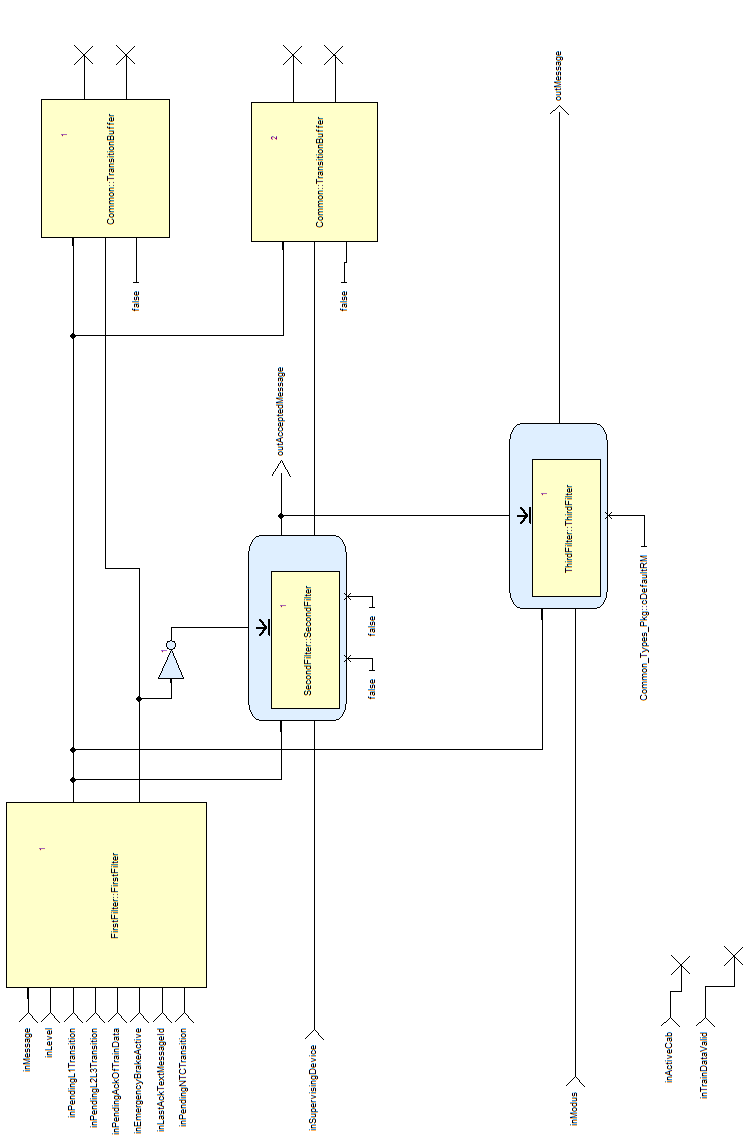
\includegraphics [width=\textwidth]{images/informationfilter-high-level-rot.png}
\caption{High level overview of the InformationFilter components.}
\label{fig:InformationFilterHighLevel}
\end{figure}

\paragraph{Interface}

For an overview of the interface of this internal component we refer to the SCADE model (cf.~link above) respectively the SCADE generated documentation.
